\documentclass[aspectratio=169,11pt]{beamer}

% Shared style (ib-tutorials.sty at the repo root).
\makeatletter\def\input@path{{./}{../}}\makeatother
\usepackage{ib-tutorials}

\usepackage[utf8]{inputenc}
\usepackage{amsmath,amssymb}
\usepackage{booktabs}
\usepackage{array}
\newcolumntype{L}[1]{>{\raggedright\arraybackslash}p{#1}}
\usepackage{graphicx}
\graphicspath{{../pictures/3-ibamr-fundamentals/}{pictures/3-ibamr-fundamentals/}}
\usepackage{xcolor}
\usepackage{listings}
\usepackage{tikz}
\usetikzlibrary{arrows.meta,positioning,shapes.geometric,fit,calc,decorations.pathmorphing}
\usepackage{hyperref}

\newcommand{\sourcecredit}[1]{\vfill\begin{flushright}\tiny\textcolor{DarkGray}{#1}\end{flushright}}

\lstset{
  basicstyle=\ttfamily\scriptsize\color{BlackGray},
  keywordstyle=\color{NavyBlue}\bfseries,
  commentstyle=\color{DarkGray}\itshape,
  stringstyle=\color{OliveGreen},
  showstringspaces=false,
  columns=fullflexible,
  keepspaces=true,
  breaklines=true,
  breakindent=1em,
  frame=single,
  framerule=0.4pt,
  rulecolor=\color{LightGray},
  backgroundcolor=\color{LightGray!30},
  xleftmargin=0.25em,
  xrightmargin=0.25em
}
\lstdefinestyle{shell}{morecomment=[l]{\#}}
\lstdefinestyle{input}{morecomment=[l]{//}}
\lstdefinestyle{matlab}{morecomment=[l]{\%}}
\lstdefinestyle{python}{morecomment=[l]{\#}}
\lstdefinestyle{data}{}
\lstdefinestyle{tiny}{basicstyle=\ttfamily\tiny\color{BlackGray}}
\lstdefinestyle{inputtiny}{morecomment=[l]{//},basicstyle=\ttfamily\tiny\color{BlackGray}}
\lstdefinestyle{matlabtiny}{morecomment=[l]{\%},basicstyle=\ttfamily\tiny\color{BlackGray}}
\lstdefinestyle{pythontiny}{morecomment=[l]{\#},basicstyle=\ttfamily\tiny\color{BlackGray}}
\lstdefinestyle{shelltiny}{morecomment=[l]{\#},basicstyle=\ttfamily\tiny\color{BlackGray}}
\lstdefinestyle{cpp}{language=C++,morecomment=[l]{//}}
\lstdefinestyle{cpptiny}{language=C++,morecomment=[l]{//},basicstyle=\ttfamily\tiny\color{BlackGray}}
\lstdefinestyle{cmake}{morecomment=[l]{\#}}
\lstdefinestyle{cmaketiny}{morecomment=[l]{\#},basicstyle=\ttfamily\tiny\color{BlackGray}}

\title[Tour of the upstream examples]{Tour of the upstream examples}
\subtitle{What the examples that ship with IBAMR do: the IB, CIB, ConstraintIB, Navier--Stokes, advection--diffusion, level-set, multiphase, complex-fluid and other suites, how to build them, and which ones ran}
\author[Miller]{Laura A. Miller}
\institute[UArizona]{Department of Mathematics, University of Arizona}
\date{Using IB Software \textbullet\ Part III \textbullet\ Chapter 15}

\begin{document}

% 1
\begin{frame}[plain]
\maketutorialtitlepanel{%
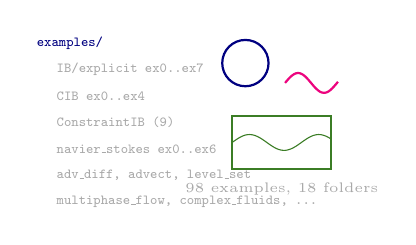
\begin{tikzpicture}[scale=0.84]
  \node[font=\tiny\ttfamily,text=NavyBlue,anchor=west] at (0,2.5) {examples/};
  \node[font=\tiny\ttfamily,text=DarkGray,anchor=west] at (0.3,2.1) {IB/explicit ex0..ex7};
  \node[font=\tiny\ttfamily,text=DarkGray,anchor=west] at (0.3,1.7) {CIB ex0..ex4};
  \node[font=\tiny\ttfamily,text=DarkGray,anchor=west] at (0.3,1.3) {ConstraintIB (9)};
  \node[font=\tiny\ttfamily,text=DarkGray,anchor=west] at (0.3,0.9) {navier\_stokes ex0..ex6};
  \node[font=\tiny\ttfamily,text=DarkGray,anchor=west] at (0.3,0.5) {adv\_diff, advect, level\_set};
  \node[font=\tiny\ttfamily,text=DarkGray,anchor=west] at (0.3,0.1) {multiphase\_flow, complex\_fluids, ...};
  \draw[NavyBlue,thick] (3.3,2.2) circle (0.35);
  \draw[RubineRed,thick] plot[domain=3.9:4.7,samples=30] (\x,{1.9+0.15*sin(deg(8*(\x-3.9)))});
  \draw[OliveGreen,thick] (3.1,0.6) rectangle (4.6,1.4);
  \draw[OliveGreen,thin] plot[domain=3.1:4.6,samples=40] (\x,{1.0+0.12*sin(deg(6*(\x-3.1)))});
  \node[font=\tiny,text=DarkGray] at (3.85,0.3) {98 examples, 18 folders};
\end{tikzpicture}}
\end{frame}

% 2
\begin{frame}{Learning goals}
\label{fr:goals}
\footnotesize By the end of this chapter you should be able to:
\begin{enumerate}
  \item find your way round the \code{examples/} folder of the IBAMR source tree: the eighteen suites, what physics and which solver class each one exercises, and which of this series' chapters goes with it;
  \item say what each of the eight basic IB examples does, which files it needs, how long it runs, and what to look at in VisIt; the same for the CIB and Navier--Stokes suites, and in outline for the rest;
  \item build the examples two ways: inside IBAMR's own build tree with \code{make examples-IB} or \code{make IB-ex1}, and outside it, against an installed (autoibamr) IBAMR, with the plain \code{CMakeLists.txt} of this series;
  \item map the example names of the 2013 and 2015 course decks onto today's folders, and know which three statements of the older decks were wrong;
  \item pick the example nearest to your own problem as a starting point, and know what it will cost to run.
\end{enumerate}
\begin{punchbox}
\footnotesize Everything in chapters 5--14 was built on these examples. This chapter is the map: forty of them were built and started for it on IBAMR 0.19.0, and the table on slides \ref{fr:ran} and \ref{fr:ran2} says what happened.
\end{punchbox}
\end{frame}

% 3
\begin{frame}{How this chapter was checked}
\label{fr:checked}
\begin{itemize}\footnotesize
  \item The example list, the files, the input parameters, the README texts and the classes each program creates are read from the IBAMR 0.19.0 source tree (\code{examples/}), not from memory or from the older decks.
  \item Forty of the examples (every 2D one of the IB, CIB, Navier--Stokes, advection--diffusion, level-set and complex-fluid suites, one or two of each other suite, and the 3D ones that are cheap) were built against the installed 0.19.0 with a plain \code{CMakeLists.txt} and run for up to two minutes on two ranks; slides \ref{fr:ran} and \ref{fr:ran2} report every build and run, including the ones that did not work that way. The gallery pictures are VisIt renders of those runs.
  \item The 2020 lecture \emph{What do Boyce's examples do?} (IBAMR Lecture 6, 25 slides), the 2013 \emph{IBAMR Examples} deck (18 slides; re-uploaded unchanged as the 2015 tutorial ``Boyce's Examples'') and the 2012 lab ReadMe's ``Other examples'' slide are quoted in full; where a slide was wrong about the code, it is quoted and corrected.
  \item The IBFE examples are listed here and toured in chapter 25; ConstraintIB's nine were chapter 14's.
\end{itemize}
\begin{punchbox}
\footnotesize Slide numbers refer to this deck; chapter numbers (2, 3, 5, 6, 7, 9a, 10, 11, 12, 13, 14, 16, 24, 25, 26) to the other chapters of this series.
\end{punchbox}
\end{frame}

% 4
\begin{frame}{Where to look things up}
\label{fr:lookup}
\small
\begin{itemize}
  \item \al{The tree}: \code{<autoibamr>/tmp/unpack/IBAMR-0.19.0/examples/} (chapter 2), or \url{https://github.com/IBAMR/IBAMR/tree/master/examples}.
  \item \al{Each example}: its \code{example.cpp} (the program; \code{main.cpp} in a few), \code{input2d}/\code{input3d} and their variants, the structure files, sometimes a \code{README}, a MATLAB generator or an analysis script.
  \item \al{The build}: \code{examples/CMakeLists.txt} (the \code{IBAMR\_ADD\_EXAMPLE} macro, slide \ref{fr:cmake}) and each suite's \code{CMakeLists.txt} for the target names.
  \item \al{The papers}: each README names its paper where there is one; the lectures named Bhalla et al.\ (2013) for ConstraintIB, Kallemov et al.\ (2016) for CIB, Barrett's dissertation for complex fluids, Griffith \& Lim (2012) for the rod, Zhu \& Peskin (2002) and Kim \& Peskin (2007) for the filament.
  \item \al{The lectures}: IBAMR Lecture 6 (2020), the 2013/2015 examples deck, the 2012 ReadMe (chapter 0.1's source list).
\end{itemize}
\end{frame}

% 5
\begin{frame}{The example tree in IBAMR 0.19.0 (1): structures}
\label{fr:tree}
\scriptsize
\setlength{\tabcolsep}{3pt}
\begin{tabular}{@{}llL{0.5\textwidth}l@{}}
\toprule
folder & count & what it exercises & chapters\\
\midrule
\code{IB/explicit} & 8 & the standard IB method: bands, shells, a cylinder, a filament with mass, a rod, random points, a minimal integrator, posts & 5--13, this one\\
\code{CIB} & 5 & rigid bodies by the constraint method with mobility solvers (Stokes) & this one\\
\code{ConstraintIB} & 9 & rigid and prescribed-deformation bodies by velocity correction & 14\\
\code{IBFE/explicit} & 12 & the finite-element IB method & 25\\
\code{IMP/explicit} & 1 & the immersed material point method & this one\\
\code{IIM} & 10 & the immersed interface and immersed Lagrangian--Eulerian methods (libMesh surfaces) & this one\\
\code{DLM} & 1 & distributed Lagrange multipliers: the Turek--Hron benchmark & this one\\
\code{IBLevelSet} & 7 & fully Eulerian FSI with level sets & this one\\
\bottomrule
\end{tabular}
\vspace{1mm}

\scriptsize $98$ examples in $18$ suites (the eighteenth, \code{IB}, holds only \code{explicit}). The solid-mechanics suites first; the fluid-only and multiphase suites follow on the next slide.
\end{frame}

\begin{frame}{The example tree in IBAMR 0.19.0 (2): fluids, scalars, free surfaces}
\label{fr:tree2}
\scriptsize
\setlength{\tabcolsep}{3pt}
\begin{tabular}{@{}llL{0.5\textwidth}l@{}}
\toprule
folder & count & what it exercises & chapters\\
\midrule
\code{navier\_stokes} & 7 & the fluid solver alone: exact solutions, cavities, Boussinesq convection & this one, 16\\
\code{vc\_navier\_stokes} & 4 & variable-density, variable-viscosity solver checks & this one\\
\code{adv\_diff} & 9 & a scalar advected and diffused; flux-based penalization for Neumann/Robin walls & this one, 24\\
\code{advect} & 1 & pure advection of a blob & this one\\
\code{level\_set} & 2 & level-set initialization and transport & this one\\
\code{multiphase\_flow} & 14 & air--water flows: drops, dam breaks, bodies hitting a free surface & this one\\
\code{wave\_tank} & 2 & numerical wave tanks & this one\\
\code{complex\_fluids} & 5 & Oldroyd-B fluids & this one\\
\code{fe\_mechanics} & 1 & solid mechanics alone (Cook's membrane) & this one\\
\bottomrule
\end{tabular}
\vspace{1mm}

\scriptsize $98$ examples. \code{examples/CMakeLists.txt} lists the suites in the order \code{CIB ConstraintIB DLM IB IBFE IBLevelSet IMP IIM adv\_diff advect complex\_fluids fe\_mechanics level\_set multiphase\_flow navier\_stokes vc\_navier\_stokes wave\_tank}; the 2020 lecture's slide 2 named five of them, ``IB -- basic immersed boundary examples, IBFE -- Hybrid IB/Finite element examples, Constraint IB -- Bhalla et al., 2013, CIB -- Kallemov et al., 2016, Complex fluids -- Barrett dissertation'', with a screenshot of the folder listing.
\end{frame}

% 6
\begin{frame}{Three generations of ``Boyce's examples'' in the course}
\label{fr:gens}
\footnotesize
\begin{itemize}
  \item \al{2012, the lab ReadMe, slide 10 ``Other examples'':} ``There are many other examples that Boyce has put together in the examples folder. You can go into each folder, make the examples, and run them. IB are immersed boundary examples, IBFE are immersed boundary -- finite element, adv\_diff include advection diffusion, etc. For example, do \code{cd IB}, \code{cd staggered\_grid}, \code{cd explicit}, \code{make examples}, \code{cd ex0}, \code{make main2d}, \code{./main2d input2c}'' (the last is a typo for \code{input2d}; the path \code{IB/staggered\_grid/explicit} is the 2012 layout, today \code{IB/explicit}).
  \item \al{2013, \emph{IBAMR Examples} (MATH 769, April 4, 2013; 18 slides), re-uploaded in 2015 as tutorial 12 ``What do Boyce's examples do?'':} one slide each for \code{IB/explicit} ex1--ex4 (the old numbering, slide \ref{fr:oldnames}), \code{navier\_stokes} ex0, ex2, ex4, ex5, \code{advect} and \code{adv\_diff/ex0}, with VisIt screenshots and input excerpts.
  \item \al{2020, IBAMR Lecture 6 \emph{What do Boyce's examples do?} (25 slides):} how to run them on the UA cluster (slides 3--5), \code{IB/explicit} ex0--ex5, \code{CIB} ex0--ex4, ConstraintIB (six slides, chapter 14), and ``More examples next week: For next week, I'd like to go through the non-Newtonian and level set examples. Then I'd like to revisit the IBFE ones. I encourage you to run and look at examples that are related to your target applications and discuss them next week.''
\end{itemize}
\begin{punchbox}
\footnotesize The suite grew from about 25 examples in 2013 to 98 in 0.19.0; this chapter covers all 98 in outline and the ones the lectures opened in detail.
\end{punchbox}
\end{frame}

% 7
\begin{frame}[fragile]{Building them in 2020: copy, Makefile, script}
\label{fr:build2020}
\begin{columns}[T,onlytextwidth]
\begin{column}{0.5\textwidth}
\footnotesize ``Running Boyce's examples. You will want to copy the examples folder to your xdisk space. \code{\$ pwd} \code{/groups/lauram9/ib16/Code/IBAMR} \code{\$ cp -r examples /xdisk/lauram9/lauram9/examples}. You will also want to move a Makefile and a script.sh into each example folder you plan to run. Text for the Makefile is on the next slide and also on github.'' (2020, slide 3)
\begin{lstlisting}[style=shelltiny]
# slide 4, "Makefile text" (the parts that matter)
IBAMR_SRC_DIR = /groups/lauram9/ib16/Code/IBAMR
IBAMR_BUILD_DIR = /groups/lauram9/ib16/Code/ibamr-objs-opt
LIBSNEW = $(LIBS) -lnetcdf -lcurl
include $(IBAMR_BUILD_DIR)/config/make.inc
SOURCES = example.cpp
OBJS = example.o
main2d:
	if (test -f stamp-3d); then $(MAKE) clean; fi
	touch stamp-2d
	$(MAKE) PDIM=2 main-2d
main-2d: $(IBAMR_LIB_2D) $(IBTK_LIB_2D) $(OBJS) $(SOURCES)
	$(CXX) $(CXXFLAGS) $(LDFLAGS) $(OBJS) \
	$(IBAMR_LIB_2D) $(IBTK_LIB_2D) $(LIBSNEW) -DNDIM=$(PDIM) -o main2d
\end{lstlisting}
\end{column}
\begin{column}{0.48\textwidth}
\begin{lstlisting}[style=shelltiny]
# slide 5, "Sample script text"
#!/bin/bash
#SBATCH --job-name=CIB_Examples
#SBATCH --ntasks-per-node=16
#SBATCH --nodes=1
#SBATCH --time=1:00:00
#SBATCH --partition=standard
#SBATCH --account=lauram9
#SBATCH --output=IBAMR2D.output

mpirun ./main2d input2d
\end{lstlisting}
\scriptsize That Makefile is the autotools era (chapter 3): it includes \code{make.inc} from an IBAMR \emph{build} directory and links the 2D or 3D library by hand; ``Be sure to change all of the 2's in the Makefile to 3's'' (slides 7, 8) for a 3D example. The commented-out paths in it point at the 2018 dogwood module at UNC. Both the source tree and the build directory it names are gone; chapter 2's autoibamr puts the sources in \code{<autoibamr>/tmp/unpack/IBAMR-0.19.0} and the library in \code{<autoibamr>/packages/}.
\end{column}
\end{columns}
\end{frame}

% 8
\begin{frame}[fragile]{Building them now (1): inside IBAMR's own build tree}
\label{fr:cmake}
\begin{columns}[T,onlytextwidth]
\begin{column}{0.52\textwidth}
\begin{lstlisting}[style=cmaketiny]
# examples/CMakeLists.txt (IBAMR 0.19.0), the helper every suite uses
# IBAMR_ADD_EXAMPLE(
#   TARGET_NAME       "IBFE-ex0"
#   OUTPUT_DIRECTORY  "${CMAKE_BINARY_DIR}/examples/IBFE/explicit/ex0"
#   OUTPUT_NAME       main2d
#   EXAMPLE_GROUP     examples-IBFE
#   SOURCES           "example.cpp"
#   REQUIRES          IBAMR_HAVE_LIBMESH
#   LINK_TARGETS      IBAMR2d
#   INPUT_FILES       input2d cylinder2d.vertex petsc_options.dat
#   )
ADD_CUSTOM_TARGET(examples)
SET(EXAMPLE_DIRECTORIES CIB ConstraintIB DLM IB IBFE IBLevelSet IMP IIM adv_diff
  advect complex_fluids fe_mechanics level_set multiphase_flow navier_stokes
  vc_navier_stokes wave_tank)
    ADD_EXECUTABLE("${EX_TARGET_NAME}" EXCLUDE_FROM_ALL ${EX_SOURCES})
    FOREACH(_input_file ${EX_INPUT_FILES})
      CONFIGURE_FILE("${_input_file}" "${EX_OUTPUT_DIRECTORY}" COPYONLY)
    ENDFOREACH()
  ELSE()
    MESSAGE(STATUS "Example ${EX_TARGET_NAME} requires libMesh - skipping")
\end{lstlisting}
\end{column}
\begin{column}{0.46\textwidth}
\scriptsize In the directory where IBAMR itself was configured with CMake (autoibamr's \code{tmp/build/v0.19.0} while it exists, or your own):
\begin{lstlisting}[style=shelltiny]
make examples          # every example (EXCLUDE_FROM_ALL: not built by default)
make examples-IB       # one suite
make IB-ex1            # one example
cd examples/IB/explicit/ex1 && mpirun -np 4 ./main2d input2d
\end{lstlisting}
\scriptsize The executable is named \code{main2d} or \code{main3d} and placed in \code{<build>/examples/<suite>/<ex>/} together with the \code{INPUT\_FILES} and \code{EXTRA\_FILES} the suite's \code{CMakeLists.txt} lists (inputs, vertex files, \code{petsc\_options.dat}, MATLAB scripts), so you run there, not in the source tree. Examples whose \code{REQUIRES} is not met (libMesh for IBFE, IIM, parts of multiphase and complex fluids) are skipped with the message shown. Chapter 2 timed \code{make -j4 IB-ex1} at 28 s.
\end{column}
\end{columns}
\end{frame}

% 9
\begin{frame}[fragile]{Building them now (2): outside the tree, against an installed IBAMR}
\label{fr:cmake2}
\begin{columns}[T,onlytextwidth]
\begin{column}{0.5\textwidth}
\begin{lstlisting}[style=cmaketiny]
# CMakeLists.txt dropped into a copy of any example folder (this series' form, chapter 3)
cmake_minimum_required(VERSION 3.15...3.30)
project(tour LANGUAGES C CXX)
find_package(IBAMR 0.16.0 REQUIRED)
add_executable(main2d example.cpp)          # plus the example's other .cpp files
target_link_libraries(main2d PRIVATE IBAMR::IBAMR2d)
\end{lstlisting}
\begin{lstlisting}[style=shelltiny]
cp -r $IBAMR_SRC/examples/IB/explicit/ex1 ~/work/ex1 && cd ~/work/ex1
# write the CMakeLists.txt above (replace the suite's own, which needs the macro)
cmake -S . -B build -DCMAKE_BUILD_TYPE=Release
cmake --build build -j 4
mpirun -np 4 ./build/main2d input2d
\end{lstlisting}
\end{column}
\begin{column}{0.48\textwidth}
\footnotesize This is how the forty examples of slides \ref{fr:ran} and \ref{fr:ran2} were built: copy the folder, replace its \code{CMakeLists.txt} (the upstream one calls \code{IBAMR\_ADD\_EXAMPLE} and links \code{IBAMR2d}, names that exist only inside IBAMR's build), list every \code{.cpp} of the folder except helper programs, and link \code{IBAMR::IBAMR2d} or \code{IBAMR::IBAMR3d}.
\scriptsize autoibamr deletes its build tree after installing unless told to keep it, so on a machine set up by chapter 2 this route is usually gone; this route always works. What to leave out and where to run: next slide.

\end{column}
\end{columns}
\end{frame}

\begin{frame}{Building them now (3): what to leave out, and where to run}
\label{fr:cmake3}
\footnotesize
\begin{itemize}
  \item \al{Helper programs} are separate executables upstream: \code{convergence\_tester.cpp} (\code{navier\_stokes/ex1}, \code{complex\_fluids/ex2}), the \code{*Gen.cpp} vertex generators of \code{multiphase\_flow} (``This file is automatically generated by the build process''), \code{write\_ascii.cpp} (\code{adv\_diff/ex8}). Leave them out of \code{main2d}, or build each as its own target.
  \item \al{Inputs with suffixes} (\code{input2d.cylinder}, \code{input2d.plate}, \code{input2d\_CaseA}) are passed by name.
  \item \al{\code{petsc\_options.dat}} (CIB) is read from the working directory.
  \item The 3D examples need \code{main3d} and \code{IBAMR::IBAMR3d}; the same \code{example.cpp} compiles for both (\code{NDIM} comes from the library target).
\end{itemize}
\vspace{1mm}

\footnotesize The same six lines serve every suite; the forty builds of slides \ref{fr:ran} and \ref{fr:ran2} were made by a script that writes them, lists the folder's \code{.cpp} files minus the helpers, and runs \code{cmake} (\code{wsl/final/run\_tour.sh} in this series' working files).
\end{frame}

% 10
\begin{frame}{\code{IB/explicit} (1): ex0, the pressurized band made in code}
\label{fr:ib01}
\footnotesize \al{ex0, a pressurized band.} ``This is an example of a pressurized rubber band. The figure shows a color map of the pressure and the resulting velocity vectors. Input2d was used in this simulation. There is also input2d.shell and input2d.shell\_circum\_fibers that you can use to make different kinds of rubber bands.'' (2020, slide 6)
\begin{itemize}\scriptsize
  \item no \code{.vertex} file: the band is generated in \code{example.cpp} by \code{IBRedundantInitializer}, which takes a function that returns the points and springs (the one initializer that needs no files; chapter 6 named the other);
  \item a $1$ m periodic box, $64\times64$ cells, one level; $\mu = 10^{-2}$, $\rho = 1$, stiffness \code{K = 1}; the run is $0.55$ s in $2{,}200$ steps (\code{DT = 1.6e-2*DX}), eight seconds on two ranks;
  \item \code{input2d.shell} and \code{.shell\_circum\_fibers}: a band of finite width \code{W = 0.0625} with radial, or radial and circumferential, springs.
\end{itemize}
\vspace{1mm}

\scriptsize Why it matters: every other example starts from files, and chapter 6 is about those files; ex0 shows the one way round them, which is also the way a generator written in C++ (chapter 12's 3D cases) hands points to IBAMR.
\end{frame}

\begin{frame}{\code{IB/explicit} (2): ex1, the bouncing ellipse and the shells}
\label{fr:ib1}
\footnotesize \al{ex1, the bouncing ellipse.} ``This is an example of a bouncing rubber band initialized as an ellipse. The figure shows a color map of the pressure and the resulting velocity vectors. Input2d was used in this simulation. As in the other example, there is input2d.shell and input2d.shell\_circum\_fibers. There is also a 3D shell you run with input3d. Be sure to change all of the 2's in the Makefile to 3's.'' (slide 7)
\begin{itemize}\scriptsize
  \item the same box and fluid as ex0, but the structure comes from files: \code{curve2d\_64} to \code{\_512} (\code{.vertex}, \code{.spring}) from \code{generate\_curve2d.m}, the shells \code{shell2d\_*} and \code{shell2d\_radial\_*} from \code{generate\_shell2d.m}, and \code{sphere3d} for \code{input3d} (three levels, $\mu = 0.005$, $2.4$ s);
  \item the 2013 deck's ``ex1 -- Bouncing rubberband'' and ``ex1 -- Bouncing shell'' are this example: ``a band that resists stretching. It has periodic boundary conditions'' and ``The structure is reinforced in the radial and circumferential directions. The shell starts as an ellipse and bounces around a circular shape. .spring and .vertex files are used to make the structure.'';
  \item this series' IB/01 (chapters 3, 5, 6) is ex1's band with its own files; chapter 16 uses ex1's four resolutions for a convergence test.
\end{itemize}
\end{frame}

% 11
\begin{frame}[fragile]{\code{IB/explicit} (3): ex2, flow past a cylinder or a sphere}
\label{fr:ib2}
\begin{columns}[T,onlytextwidth]
\begin{column}{0.5\textwidth}
\scriptsize ``This is an example of flow past a cylinder. The example includes analysis files to calculate the Strouhal number. The figure shows a color map of the vorticity and the resulting velocity vectors. Input2d.cylinder was used in this simulation. There is also a 3D cylinder and a sphere with corresponding input files. Be sure to change all of the 2's in the Makefile to 3's.'' (2020, slide 8)
\end{column}
\begin{column}{0.48\textwidth}
\begin{itemize}\scriptsize
  \item \code{input2d.cylinder}: $R = 0.5$, $\mathrm{Re} = 200$ (\code{MU = 2R/Re}), five levels refined by 2 from $N = 16$; the inflow ramps up smoothly (next slide); \code{END\_TIME = 300}: a Puma job (chapter 1), not a laptop run; two minutes on two ranks gave $9{,}649$ steps (slide \ref{fr:ran});
  \item the tethering is in the input, not a \code{.target} file: \code{uniform\_target\_stiffness} and \code{uniform\_target\_damping} under the structure's block of \code{IBStandardInitializer} (chapter 9a's keys);
  \item \code{input2d.cylinder\_stabilized}: $\mathrm{Re} = 5000$ with the stabilized convective operator;
  \item \code{input3d.cylinder}, \code{input3d.sphere} (and \code{.cylinder.test}, $0.1$ s): a $16$ m box, two levels, $\mathrm{Re} = 100$ and $200$; vertex files from $32$ to $1024$ points across;
  \item \code{compute\_St.m}: the Strouhal number from the lift history (chapter 11).
\end{itemize}

\end{column}
\end{columns}
\end{frame}

\begin{frame}[fragile]{\code{IB/explicit} (3b): ex2 in the 2013 deck, and the ramped inflow}
\label{fr:ib2b}
\footnotesize 2013, slides 4--5: ``This was run with input2D, and it's tethered in place. Other options include a 3D cylinder and sphere. 3D sphere and cylinder flow also available. Target stiffness and damping included. Done in a way that doesn't use .target file. `Fancy' boundary conditions in 2D. U1 has prescribed inflow that is a function of time, the other boundaries are Neumann. U2 is zero on top and bottom, is function of time and position on the inflow, and has Neumann outflow.''
\vspace{1mm}

\begin{lstlisting}[style=inputtiny]
// input2d.cylinder: the ramped inflow on the left side (chapter 7)
gcoef_function_0 = "(tanh((t-t_half)/tau)+tanh(t_half/tau))/(1+tanh(t_half/tau))"
\end{lstlisting}
\footnotesize The ramp is chapter 7's time-dependent Dirichlet value: the inflow speed rises from $0$ to $1$ over about \code{tau} around \code{t\_half}, so that the cylinder is not hit by an impulsive start (chapter 16's first rule). The 2013 deck's `fancy' boundary conditions are these: a prescribed inflow on the left, zero normal velocity top and bottom, and Neumann outflow on the right.
\end{frame}

% 12
\begin{frame}[fragile]{\code{IB/explicit} (4): ex3, the tethered filament with mass}
\label{fr:ib3}
\begin{columns}[T,onlytextwidth]
\begin{column}{0.46\textwidth}
\footnotesize ``This is an example of flow past a flexible, tethered filament. The figure shows a color map of the vorticity and the resulting velocity vectors. This example was inspired by a paper by Zhu and Peskin. Go to the google drive papers folder to find it.'' (2020, slide 9)
\vspace{1mm}

\scriptsize 2013, slides 6--9: ``Inspired from an experiment. Mass was necessary to induce flapping. This simulation should flap at higher Re or higher mass.'' ``2D flow over a fiber with mass that resists bending and stretching and is tethered at the top. Boundary conditions allow flow in the y-direction. U1 is fixed on all sides to zero. U2 is set to Neumann B.C.'s. Flow is generated due to the effect of gravity. This comes from a `forcing function' in the input file.'' ``The boundary mass is added in an older way (no .mass files are used).'' ``Penalty IB method. This specific application is described in Zhu and Peskin. A `.mass' file is used to specify any additional mass associated with the IB points. For such files to have any effect, it is necessary that the IB solver be run in `penalty-IB' mode.''
\end{column}
\begin{column}{0.52\textwidth}
\begin{lstlisting}[style=inputtiny]
// input2d (0.19.0): the lines the 2013 deck quoted, still there
ForcingFunction {
   function_0 = "0.0"
   function_1 = "-g*rho*( 1 + (F-1)*exp(-400*t) - F*exp(-600*t) )"
}
IBStandardInitializer {
   structure_names = "fila_256"
   fila_256 {
      level_number = MAX_LEVELS - 1
      ds = 3.84 / NFINEST
      uniform_spring_stiffness = spring_stiffness
      uniform_spring_rest_length = ds
      uniform_beam_bend_rigidity = bend_rigidity*ds/(ds^4)
      uniform_bdry_mass = bdry_mass_density*ds
      uniform_bdry_mass_stiffness = bdry_mass_stiffness
   }
}
\end{lstlisting}
\scriptsize \code{example.cpp} creates \code{PenaltyIBMethod} (chapter 13): the ``older way'' of 2013 is the \code{uniform\_bdry\_mass} keys, which give every point a massive copy without a \code{.mass} file. The fluid is a gas ($\rho = 3\times10^{-4}$, $\mu = 1.2\times10^{-3}$, ``Re=210''), gravity $980$ cm/s$^2$ ramps up through the forcing function, and five levels refined by 2 from $N = 16$ in a $9$ cm box. \code{DT = 0.128/NFINEST\^{}2} is $2\times10^{-6}$ s: the $1.2$ s run is $600{,}000$ steps, a cluster job; two minutes on a laptop gave slide \ref{fr:ran}'s count. Files for $256$, $512$ and $1024$ points.
\end{column}
\end{columns}
\end{frame}

% 13
\begin{frame}{\code{IB/explicit} (5): ex4, the Kirchhoff rod}
\label{fr:ib45}
\footnotesize \al{ex4.} ``This is an 3D example of a rubber band that starts out as a circle that is loaded with torsion. The infinitely thin boundary can apply rotational forces to the fluid. Eventually the rubber band twists in 3D as seen in this snapshot. Griffith, Boyce E and Lim, Sookkyung. Simulating an Elastic Ring with Bend and Twist by an Adaptive Generalized Immersed Boundary Method. Communications in computational physics, 08/2012, Volume 12, Issue 2, pp. 433--461.'' (2020, slide 10)
\vspace{1mm}

\scriptsize 2013, slide 11: ``IB/explicit/ex4 - Kirchoff Rods. 3D flow around a 1D ring that has an intrinsic curvature and twist. The fluid-rod interaction problem is solved by the generalized immersed boundary method combined with the Kirchhoff rod theory. The files include .rod and .director files.'' (``Kirchoff'' is the slide's spelling; the links it gave, to math.nyu.edu and pof.aip.org, are dead.)
\vspace{1mm}

\scriptsize Files: \code{curve3d\_64.vertex}, \code{.rod}, \code{.director} from \code{generate\_mesh3d.m}; \code{example.cpp} uses \code{IBKirchhoffRodForceGen} in place of \code{IBStandardForceGen}. A $10$ cm box, three levels refined by 2 to $64$ cells, $\mu = 0.01$, $100$ s of run: a 3D cluster job (slide \ref{fr:ran} has the two-minute start).
\end{frame}

\begin{frame}{\code{IB/explicit} (6): ex5, which is not what the lecture said}
\label{fr:ib5}
\footnotesize \al{ex5, corrected.} ``This example includes a bunch of immersed boundary points that each move with their own behavior. The vertices and their x, y-coordinates are outputted, but the flow fields are not.'' (2020, slide 11)
\vspace{1mm}

\footnotesize That is not what ex5 is. Its input begins with ``random-number generator parameters'' (\code{SEED}), a temperature \code{kT = 1.0}, and the fluid parameters; \code{example.cpp} creates \code{INSStaggeredStochasticForcing}: it is \emph{fluctuating hydrodynamics}, a fluid with thermal noise in which a cloud of free IB points (\code{points2d.vertex}, \code{points3d.vertex}, with no springs) diffuses by Brownian motion. The points have no behaviour of their own; the fluid is random. The flow fields \emph{are} written: \code{viz\_writer = "VisIt","Silo"} with \code{VISIT\_DUMP\_INTERVAL = 10}, and the positions go to ASCII \code{X.*} files besides (chapter 11's format). \code{DT = 10.0} and \code{END\_TIME = N\_STEPS*DT}: the run is counted in steps, not seconds.
\vspace{1mm}

\scriptsize What the lecturer saw, a scatter of dots and no flow, was VisIt showing the Lagrangian mesh alone (slide 11's picture): the fluid data were there in \code{viz\_IB2d}.
\end{frame}

% 14
\begin{frame}{\code{IB/explicit} (7): ex6, a minimal integrator in two files}
\label{fr:ib67}
\footnotesize \al{ex6, a minimal IB integrator.} The band of ex1 (\code{curve2d\_64} to \code{\_512}, \code{generate\_curve2d.m}, the same input) run by \code{IBSimpleHierarchyIntegrator}, a time integrator written in the example's own two files (\code{IBSimpleHierarchyIntegrator.cpp}, \code{.h}) instead of the library's \code{IBExplicitHierarchyIntegrator}: forward Euler for the points, the standard spread and interpolate, and nothing else. It is the shortest complete statement of chapter 5's algorithm in IBAMR's own terms, about two hundred lines, and the place to start if you ever need an integrator of your own. Eight seconds for the $2{,}200$ steps.
\vspace{1mm}

\footnotesize Read \code{IBSimpleHierarchyIntegrator.cpp} next to chapter 5's slides: \code{integrateHierarchy} spreads the force, solves the fluid, interpolates the velocity and moves the points, in that order and nothing else.
\end{frame}

\begin{frame}{\code{IB/explicit} (8): ex7, posts in 3D with a scalar}
\label{fr:ib7}
\footnotesize \al{ex7, posts in 3D with a scalar.} README: ``This is a tutorial example used to track the IB coordinates of a single post which undergoes prescribed motion. In this example, the IB coordinates of the post are prescribed to lie and move along the level set of a cone who's radius and length is set by the post\_deflection\_radius and post\_length either in the input file, or using the default values as specified in the example.cpp file. After running the executable associated with this example, a `IBCoordinates.txt' file is generate whose columns correspond to the relevant Lagrangian index as specified in the .vertex file and the Eulerian x,y,z coordinates. \ldots The MATLAB script `generate\_posts.m' is used to generate the IB points of the posts located at the center of the square domain. \ldots Notice that a number of problem parameters are currently `hard coded' in this script.''
\vspace{1mm}

\scriptsize A $1\times1\times0.25$ cm box of water, three levels, an advected--diffused scalar (\code{D = 1e-3}, \code{AdvDiffSemiImplicitHierarchyIntegrator} alongside the IB solver, chapter 24), $1$ s of run; \code{posts\_128.vertex}. The README's warnings about keeping \code{NFINEST} and the domain equal in the script and the input are chapter 8a's rule.
\end{frame}

% 15
\begin{frame}{\code{CIB} (1): rigid bodies with mobility solvers}
\label{fr:cib}
\footnotesize ``CIB Examples. An Immersed Boundary Method for Rigid Bodies. Bakytzhan Kallemov, Amneet Pal Singh Bhalla, Boyce E. Griffith, and Aleksandar Donev. This paper is on the google drive. Note that it is the more recent paper for two different methods used for rigid body simulations. Some of the examples considered in this paper appear in these CIB examples.'' (2020, slide 12)
\vspace{1mm}

\footnotesize \code{CIBMethod} with \code{CIBStaggeredStokesSolver}: the rigidity constraint written as a saddle-point problem and solved with a \emph{mobility} matrix (the velocity a body gets from a force), which is why these examples ship a \code{petsc\_options.dat} and keys like \code{STOKES\_TOL}, \code{DELTA} (``regularization parameter for mobility matrix'') and \code{VISC\_CFL = 1E-16}. Three of the five are steady Stokes problems that take \emph{one} time step: ``this example only runs one DT'' (slide 13) is by design.
\vspace{1mm}

\footnotesize Where it sits: chapter 14's \code{ConstraintIBMethod} corrects velocities and needs no linear solve of its own; \code{CIBMethod} solves for the constraint forces exactly, which is what a suspension of many rigid particles at zero Reynolds number needs, and what makes a single CIB step expensive. The paper: B. Kallemov, A. P. S. Bhalla, B. E. Griffith and A. Donev, \emph{An immersed boundary method for rigid bodies}, Commun.\ Appl.\ Math.\ Comput.\ Sci.\ 11 (2016) 79--141.
\end{frame}

\begin{frame}{\code{CIB} (2): the five examples}
\label{fr:cib2}
\scriptsize
\setlength{\tabcolsep}{3pt}
\begin{tabular}{@{}lL{0.9\textwidth}@{}}
\toprule
ex0 & ``This example shows how to set various solvers for a fully prescribed kinematics for a 2d body.'' (README). Lecture: ``basically a cylinder in 2D that rotated in a prescribed way. I only had two time steps that wrote to a visualization file, and checking the input file this example only runs one DT.'' $\rho = 0$, $\mu = 1$: Stokes.\\
ex1 & ``a mixture of prescribed and free DOFs for two bodies. The outer shell (structure 0) moves relative to the inner sphere (structure 1). The mobility matrices \ldots are formed independently and are distributed to different processors \ldots Forces and torques on both spheres (strct\_id\_0) and the inner sphere (strct\_id\_1) are computed via control volume analysis.'' 3D; one step. Lecture: ``Stokes flow between two concentric spherical shells.''\\
ex2 & ``A 2d plate is dragged with an imposed velocity for a certain time, after which it translates freely but with locked rotational motion.'' $\mathrm{Re} = 20$, $15$ s; \code{input2d.plate.amr} adds a level. Lecture: ``This example outputs many times. In the 2 hour debug queue I don't see rotation.'' (none is allowed: the rotation is locked.)\\
ex3 & flow through a nozzle, $\mathrm{Re} = 10$, $100$ steps; no README. Lecture: ``The snapshot shows the velocity vectors and the color map shows the pressure. This example comes directly from the paper in the section on flow through a nozzle.''\\
ex4 & a falling sphere, 3D, $\rho = 2$, $50$ s (\code{input3d.test.long}: $1.8$ s); \code{check\_sol.m}. Lecture: ``The movement of the sphere is driven by gravity. I don't believe this example is in the paper, look at the code to see how it is handled.''\\
\bottomrule
\end{tabular}
\end{frame}

% 16
\begin{frame}{\code{ConstraintIB}: chapter 14's nine, in one line each}
\label{fr:constraintib}
\footnotesize The constraint method of Bhalla et al.\ (2013), velocity correction without mobility matrices; the lecture spent six slides on them and chapter 14 ran three.
\begin{center}
\scriptsize
\setlength{\tabcolsep}{3pt}
\begin{tabular}{@{}llL{0.5\textwidth}l@{}}
\toprule
folder & dim & what & this series\\
\midrule
\code{stokes\_first\_problem} & 2D & a plate started impulsively (paper 7.1.1); prescribed & --\\
\code{moving\_plate} & 2D & a plate dragged across the fluid at $\mathrm{Re} = 20$ (7.1.2); prescribed, velocity by a C callback & --\\
\code{oscillating\_rigid\_cylinder} & 2D & a disc oscillating at $\mathrm{Re} = 100$, $\mathrm{KC} = 5$ (7.1.4); prescribed & ConstraintIB/01\\
\code{flow\_past\_cylinder} & 2D & a disc towed at constant speed; prescribed & --\\
\code{impulsively\_started\_cylinder} & 2D & a disc given a body-force impulse; free (7.2.2) & ConstraintIB/02\\
\code{falling\_sphere} & 3D & a sphere sinking by a gravity body force in the solid region; free & --\\
\code{eel2d} & 2D & a prescribed travelling wave, free swimming (7.3) & ConstraintIB/03\\
\code{eel3d} & 3D & the same body in 3D (\code{eelgenerator3d.cpp}, \code{InterpolationCoefs.m}) & --\\
\code{knifefish} & 3D & a knifefish with a ribbon fin (\code{KnifeFish.vertex}, 458k points, \code{RadiusAmp.dat}) & --\\
\bottomrule
\end{tabular}
\end{center}
\scriptsize Slide 24 of the lecture: ``Other examples include free swimming cases of eel swimming in 2D and 3D as well as a 3D knifefish. I have run the 2D eel, but the download is taking too long to show today. It is worth running the 3D eel and knifefish as well. There is also a falling sphere example of rigid body motion in 3D.'' The 3D eel and the knifefish are Puma jobs: $17{,}482$ and $457{,}936$ vertices.
\end{frame}

% 17
\begin{frame}{\code{navier\_stokes} (1): the fluid solver alone}
\label{fr:ns}
\scriptsize
\setlength{\tabcolsep}{3pt}
\begin{tabular}{@{}lL{0.5\textwidth}L{0.38\textwidth}@{}}
\toprule
example & what it is (0.19.0) & the 2013 deck\\
\midrule
ex0 & an exact travelling-wave solution of Navier--Stokes in a periodic box (\code{VelocityInitialConditions}, \code{PressureInitialConditions}, \code{gcoef = U}), $10$ steps; \code{input2d.forced\_flow}: the same with a body force, $0.5$ s; \code{input3d} & ``cases that can be used to test convergence against analytical solutions. Ex0 uses an exact solution with traveling waves due to forced flow. Looking at the input files will show how this is done. *I have not run all N-S examples.''\\
ex1 & the same idea with a separate \code{convergence\_tester.cpp} that compares two runs (chapter 16's grid study); $\mu = 10^{-4}$, three levels, $2$ s & --\\
ex2 & a lid-driven cavity at $\mathrm{Re} = 1000$, three levels from $N = 4$, $100$ steps; \code{analyzer.m}, \code{L1norm.m}, \code{L2norm.m} compare with the Ghia benchmark & ``This example is developing cavity flow. The left, right and bottom sides are no slip. The top has constant velocity in the x-direction and no flow in the y-direction. Warning, this outputs A LOT of data!''\\
\bottomrule
\end{tabular}
\vspace{1mm}

\scriptsize These are test programs for the fluid solver, with no structure in the box; the solver classes are the ones every IB example creates (\code{INSStaggeredHierarchyIntegrator}, or \code{INSCollocatedHierarchyIntegrator} when the input selects it), so an input block that puzzles you in an IB example can be studied here on its own.
\end{frame}

\begin{frame}{\code{navier\_stokes} (2): cavities and convection}
\label{fr:ns2}
\scriptsize
\setlength{\tabcolsep}{3pt}
\begin{tabular}{@{}lL{0.5\textwidth}L{0.38\textwidth}@{}}
\toprule
example & what it is (0.19.0) & the 2013 deck\\
\midrule
ex3 & the cavity again with \code{analyzer\_256.m}: the $256$-cell reference & --\\
ex4 & the travelling-wave flow of ex0 with an advected--diffused scalar carried along (\code{AdvDiffSemiImplicitHierarchyIntegrator}), $10$ steps; \code{input3d} & ``This is an advection diffusion example. Velocity boundary and initial conditions for an flow field with an analytical solution are in input2. Warning, this outputs A LOT of data!''\\
ex5 & Boussinesq convection: a temperature field with \code{KAPPA = 1e-6} and a buoyancy force \code{GAMMA = 1e2} (\code{BoussinesqForcing.cpp}), a $1\times2$ box, $128$ cells, $100$ steps & ``This example contains and temperature gradient and uses the Boussinesq approximation. The left, right and bottom sides are no slip. The top has constant velocity \ldots Warning, this outputs A LOT of data!'' (three pictures of the plumes)\\
ex6 & ex5 with thermal fluctuations (\code{INSStaggeredStochasticForcing}, \code{AdvDiffStochasticForcing}, \code{SEED}), $\mu = 10^{-3}$, $10$ steps & --\\
\bottomrule
\end{tabular}
\vspace{1mm}

\scriptsize ``A LOT of data'': \code{viz\_dump\_interval = 1} in the 2013 inputs. Today's inputs dump every few steps and run $10$ or $100$ steps; these are test programs, and chapter 16 uses ex1 and ex2 as the convergence examples.
\end{frame}

% 18
\begin{frame}{\code{advect} and \code{adv\_diff}: a scalar in a given flow}
\label{fr:adv}
\begin{columns}[T,onlytextwidth]
\begin{column}{0.46\textwidth}
\footnotesize \al{\code{advect}} (one example, no sub-folders): ``A blob of something with concentration Q (plotted) is advected in a given velocity field. It does not diffuse. Velocity field in input2D: \code{UFunction \{ init\_type = "UNIFORM" uniform\_u = -2.0,1.0 \}}. It has a Gaussian distribution: \code{QInit \{ init\_type = "GAUSSIAN" kappa = 0.001 \}}'' (2013, slide 17). \code{AdvectorExplicitPredictorPatchOps} alone, no fluid solver; \code{QInit.cpp}, \code{UFunction.cpp} set the blob and the velocity.
\vspace{1mm}

\footnotesize \al{\code{adv\_diff/ex0}}: ``In this example, the blob also diffuses. It is again in a prescribed flow field. See input2d'' (slide 18); the same two helper classes, \code{AdvDiffSemiImplicitHierarchyIntegrator}, and the scripts \code{converg2d}, \code{converg3d} that run it at several resolutions (chapter 16). Both finish in a second.
\end{column}
\begin{column}{0.52\textwidth}
\scriptsize
\setlength{\tabcolsep}{3pt}
\begin{tabular}{@{}lL{0.8\textwidth}@{}}
\toprule
ex1 & the scalar carried by a Navier--Stokes flow with a forcing function; $0.125$ s\\
ex2 & \code{SOLVER\_TYPE = "SEMI\_IMPLICIT"}, \code{KAPPA = 1e-2}, a Dirichlet value \code{C} on one side; $2$ s\\
ex3--ex7 & the flux-based volume-penalization method for Neumann and Robin conditions on bodies given by a level set (a cylinder, a hexagram annulus, a 1D test, an egg and a torus, a circular annulus): Poisson problems solved in one step, with READMEs that name the manufactured solutions (Sakurai et al.; Thirumalaisamy, Patankar and Bhalla, JCP 448 (2022) 110726)\\
ex8 & steady natural convection in a concentric annulus at $\mathrm{Ra} = 5\times10^4$, $\mathrm{Pr} = 0.7$, with the penalized boundaries; $10$ s; writes a temperature profile (binary; \code{write\_ascii.cpp} converts)\\
\bottomrule
\end{tabular}
\vspace{1mm}

\scriptsize These are the scalar-transport machinery that chapter 24 couples to an IB structure (oxygen round a coral, heat round a wing); ex0 and ex2 are the ones to run first.
\end{column}
\end{columns}
\end{frame}

% 19
\begin{frame}{Free surfaces (1): \code{level\_set} and \code{multiphase\_flow}}
\label{fr:multiphase}
\scriptsize
\setlength{\tabcolsep}{3pt}
\begin{tabular}{@{}L{0.2\textwidth}L{0.76\textwidth}@{}}
\toprule
\code{level\_set} ex0, ex1 & ``A test program to demonstrate initialization (via fast-sweeping method) and advection of a level set distance function''; ex1 the same by relaxation, ``to study the spatial convergence rate of the ENO subcell-fix method''. A circle in a box; seconds.\\
\code{multiphase\_flow} ex0 & ``application of a surface tension force at the boundary of a drop in static equilibrium in an ambient fluid'' (\code{SIGMA = 73}); 2D and 3D\\
ex1, ex2 & ``a circular cylinder impacting an air-water interface'' (\code{RigidBodyKinematics}, \code{input2d\_free\_fall.cyl} half-buoyant); ex2 ``uses finite element mesh for the solid body'' (libMesh)\\
ex3, ex5, ex6 & ``the importance of consistent mass and momentum transport'': a density-$10^6$ droplet convected; a collapsing water column (dam break; 2D and 3D); a droplet splashing on a thin liquid layer\\
ex4 & ``a gravitational force for a stationary water-air tank and tank filling with water''\\
\bottomrule
\end{tabular}
\vspace{1mm}

\scriptsize Air and water throughout: $\rho = 10^3$ and $1.2$, $\mu = 10^{-3}$ and $1.8\times10^{-5}$, $g = 9.81$, with \code{GRAV\_TYPE = "FLOW"} or \code{"FULL"} choosing how gravity enters; a level set marks the interface and \code{LSLocate*} classes place it.
\end{frame}

\begin{frame}{Free surfaces (2): bodies at the interface, \code{wave\_tank}, \code{vc\_navier\_stokes}}
\label{fr:multiphase2}
\scriptsize
\setlength{\tabcolsep}{3pt}
\begin{tabular}{@{}L{0.2\textwidth}L{0.76\textwidth}@{}}
\toprule
ex7, ex8, ex9 & a cylinder splashing into two fluids; a buoyant cylinder (sphere in 3D) heaving on an air-water interface; ``static equilibrium of a stationary cylinder on an air-water interface and the differences between the `full' and `flow' gravitational forces''\\
ex10--ex13 & water entry of a cylinder; a rectangular barge rolling on the interface; a half-buoyant wedge impacting the interface (2D and 3D); ``a gravity-driven 3D water column impacting a stationary obstacle''. The vertex files of ex10--ex13 ``automatically generated by the build process'' from \code{*Gen.cpp}\\
\code{wave\_tank} ex0, ex1 & ``the accuracy of Stokes first, second and fifth order waves in a numerical wave tank'' (six inputs, MATLAB comparisons); ``a second-order Stokes wave impacting a trapezoidal obstacle''\\
\code{vc\_navier\_stokes} ex0--ex3 & ``the variable-coefficient, incompressible Navier-Stokes solver yields the expected order of accuracy'': manufactured solutions with density and viscosity jumps of $10^3$ and $10^2$ (\code{ManufacturedSolution\_2D.m}, \code{extract\_error.sh}); ex2 residual convergence with a bubble; ex3 the inputs of a paper's section 6.1\\
\bottomrule
\end{tabular}
\vspace{1mm}

\scriptsize The 2020 lecture ended with ``For next week, I'd like to go through the non-Newtonian and level set examples''; that week's deck does not exist, and these two slides stand in for it. The multiphase examples with a body use \code{RigidBodyKinematics} classes of their own (not chapter 14's) and a level set for the body too.
\end{frame}

% 20
\begin{frame}{Other solids (1): \code{IBLevelSet} and \code{IIM}}
\label{fr:others}
\scriptsize
\setlength{\tabcolsep}{3pt}
\begin{tabular}{@{}L{0.18\textwidth}L{0.78\textwidth}@{}}
\toprule
\code{IBLevelSet} ex0--ex6 & fully Eulerian FSI: the body is a level set, not points. ex0 ``initialization of level set from STL mesh'' (\code{CircleMesh.msh}); ex1 ``A fully Eulerian FSI implementation of examples/ConstraintIB/oscillating\_rigid\_cylinder'' (chapter 14's ConstraintIB/01 done the other way, $26$ s); ex2 a half-buoyant cylinder hitting water; ex3 ``coupling of IBLevelSet and IBFE methods'' (a rigid rod and an elastic structure); ex4, ex5 a self-propelling pitching airfoil, one and two; ex6 a floating block with a mass-preserving level set\\
\code{IIM} ex0--ex9 & the immersed interface method and the immersed Lagrangian--Eulerian (ILE) method on libMesh surfaces (\code{.e} files): flow past a cylinder (``Sec. 4.5 of Kolahdouz et al., JCP 2020'') and a square; Hagen--Poiseuille pipe flow in 3D; a swimming thin airfoil; vortex-induced vibration of a disc; a falling sphere (glass, steel); the Turek--Hron tail; a soft disc in a cavity; a reservoir instability; a flexible plate in a flow phantom (3D)\\
\bottomrule
\end{tabular}
\vspace{1mm}

\scriptsize \code{IBLevelSet/ex1} and \code{IIM/ex0} are the same cylinder as ConstraintIB/01 and IB/explicit/ex2 done by two other methods, and the comparison is instructive.
\end{frame}

\begin{frame}{Other solids and fluids (2): \code{DLM}, \code{IMP}, \code{complex\_fluids}, \code{fe\_mechanics}}
\label{fr:others2}
\scriptsize
\setlength{\tabcolsep}{3pt}
\begin{tabular}{@{}L{0.18\textwidth}L{0.78\textwidth}@{}}
\toprule
\code{DLM} ex0 & the Turek--Hron benchmark (a $2.46\times0.41$ m channel, $D = 0.1$ m, $\mathrm{Re} = 200$) with distributed Lagrange multipliers; five inputs vary the excess mass and the stiffness\\
\code{IMP/explicit} ex0 & the immersed material point method: a \code{main.cpp} and an input, no structure files\\
\code{complex\_fluids} ex0--ex4 & Oldroyd-B fluids (\code{FLUID\_MODEL = "OLDROYDB"}): pipe flow with an exact solution (error norms printed); a four-roll mill by a background force (``As the Weissenberg number increases, singularities in the trace form at extensional points''); flow past a confined cylinder with an IBFE structure and drag output; a lid-driven cavity with a quartic lid; the four-roll mill with immersed rollers\\
\code{fe\_mechanics} ex0 & Cook's membrane, solid mechanics without fluid, 2D and 3D\\
\bottomrule
\end{tabular}
\vspace{1mm}

\scriptsize \code{complex\_fluids} is the lecture's ``non-Newtonian''; the rest are research examples that document their papers.
\end{frame}

% 21
\begin{frame}{\code{IBFE/explicit}: twelve examples for Part IV}
\label{fr:ibfe}
\footnotesize The finite-element IB examples, \code{ex0} to \code{ex11}, need libMesh (\code{REQUIRES IBAMR\_HAVE\_LIBMESH}; autoibamr builds it). They are toured in chapter 25 and used from chapter 17 on; here only the map (corrected 2026-10-15 from the sources; an earlier version of this slide listed this series' own examples under IBAMR's numbers): ex0 a pressurized elastic ring at rest, ex1 the same ring started as an ellipse, ex2 a soft plate across a box pushed by a traction difference, ex3 a soft block on the floor of a lid-driven cavity, ex4 a soft disc in a lid-driven cavity (2D and 3D), ex5 a tethered cylinder in a stream at $\mathrm{Re} = 200$ as a surface mesh or a solid (2D and 3D), ex6 the Turek--Hron beam behind a cylinder, ex7 a collapsible channel (chapter 23), ex8 a clamped beam over a slot loaded from below, ex9 a cylinder surface tethered to a prescribed position, ex10 a free rigid cylinder in Couette flow by direct forcing, ex11 flow past a fixed cylinder at $\mathrm{Re} = 200$ by direct forcing. Chapter 25 tours and runs them.
\begin{punchbox}
\footnotesize The 2020 lecture's slide 2 called them ``IBFE -- Hybrid IB/Finite element examples. Hybrid finite difference/finite element immersed boundary method''; ``Then I'd like to revisit the IBFE ones'' (slide 25) became the IBFE lecture series of Part IV.
\end{punchbox}
\end{frame}

% 22
\begin{frame}{The old names and the new (1): the 2013 and 2015 decks' IB examples}
\label{fr:oldnames}
\scriptsize
\setlength{\tabcolsep}{3pt}
\begin{tabular}{@{}L{0.3\textwidth}L{0.26\textwidth}L{0.38\textwidth}@{}}
\toprule
the 2013/2015 deck said & today (0.19.0) & notes\\
\midrule
\code{IB/explicit/ex1} -- Bouncing rubberband; ex1 -- Bouncing shell & \code{IB/explicit/ex1} (band, shells) & ex0 (the pressurized band without files) is newer\\
\code{ex2} -- Flow past cylinder (3D sphere/cylinder; targets without a \code{.target} file; time-dependent inflow) & \code{IB/explicit/ex2} & unchanged in substance; \code{compute\_St.m} added\\
\code{ex3} -- Flow past a fiber (mass ``in an older way''; penalty IB) & \code{IB/explicit/ex3} & the \code{uniform\_bdry\_mass} keys are still the way; chapter 13's \code{.mass} file is the other\\
\code{ex4} -- Kirchoff Rods (\code{.rod}, \code{.director}) & \code{IB/explicit/ex4} & 3D only\\
\bottomrule
\end{tabular}
\end{frame}

\begin{frame}{The old names and the new (2): the rest, and the dead links}
\label{fr:oldnames2}
\scriptsize
\setlength{\tabcolsep}{3pt}
\begin{tabular}{@{}L{0.3\textwidth}L{0.26\textwidth}L{0.38\textwidth}@{}}
\toprule
the 2013/2015 deck said & today (0.19.0) & notes\\
\midrule
-- & \code{ex5}, \code{ex6}, \code{ex7} & fluctuating hydrodynamics, the minimal integrator, the posts: after 2013\\
\code{navier\_stokes/ex0, ex2, ex4, ex5} & the same numbers & ex1, ex3, ex6 added; ``A LOT of data'' no longer\\
\code{advect}; \code{adv\_diff/ex0} & the same & \code{adv\_diff} ex1--ex8 added\\
IB/staggered\_grid/explicit (2012) & \code{IB/explicit} & the collocated-grid variants went; the staggered-grid solver is the one, and the inputs can still select the collocated one\\
\bottomrule
\end{tabular}
\vspace{1mm}

\scriptsize Everything the 2013 deck said about ex1--ex4 and the four Navier--Stokes examples is still true of the current folders; its screenshots (an ellipse of vorticity, a shell of springs, a cylinder wake, a filament, the cavity, the travelling waves, the Boussinesq plumes, the blob) are what you will see. Its links to \code{math.nyu.edu} and \code{pof.aip.org} are dead; the papers are Zhu \& Peskin, J.\ Comput.\ Phys.\ 179 (2002) 452--468, Kim \& Peskin, Phys.\ Fluids 19 (2007) 053103, and Lim, Ferent, Wang \& Peskin, Phys.\ Fluids 22 (2010) 024104 (the twisted-rod figure the deck reproduced).
\end{frame}

% 23
\begin{frame}{What was run for this chapter (1): IB, CIB, Navier--Stokes}
\label{fr:ran}
\scriptsize Each example copied, built with the plain \code{CMakeLists.txt} of slide \ref{fr:cmake2} against the installed 0.19.0, and run on two ranks for at most $120$ s (\code{timeout}); ``exit 124'' means the two minutes ran out with the example still going, which is a pass. Steps are what the log counted.
\vspace{1mm}

\tiny
\setlength{\tabcolsep}{2.5pt}
\begin{tabular}{@{}llllll@{}}
\toprule
example & input & build & run & steps in $\le 120$ s & viz folder\\
\midrule
\code{IB/explicit/ex0} & \code{input2d} & ok, 37 s & finished, 8 s & 2200 & \code{viz\_IB2d}\\
\code{IB/explicit/ex1} & \code{input2d} & ok, 29 s & finished, 8 s & 2200 & \code{viz\_IB2d}\\
\code{IB/explicit/ex2} & \code{input2d.cylinder} & ok, 29 s & running at 120 s & 9649 & \code{viz\_IB2d}\\
\code{IB/explicit/ex3} & \code{input2d} & ok, 34 s & running at 120 s & 10023 & \code{viz\_IB2d}\\
\code{IB/explicit/ex5} & \code{input2d} & ok, 29 s & finished, 2 s & 100 (its own loop) & \code{viz\_IB2d}\\
\code{IB/explicit/ex6} & \code{input2d} & ok, 30 s & finished, 3 s & 2200 & \code{viz\_IB2d}\\
\code{IB/explicit/ex4} & \code{input3d} & ok, 31 s & running at 120 s & 3147 & \code{viz\_IB3d}\\
\code{IB/explicit/ex7} & \code{input3d} & ok, 32 s & running at 120 s & 4527 & \code{viz\_IB3d}\\
\code{CIB/ex0} & \code{input2d} & ok, 31 s & finished, 0 s & 1 (Stokes) & \code{viz\_cylinder2d}\\
\code{CIB/ex2} & \code{input2d.plate} & ok, 32 s & running at 120 s & 199 & \code{viz\_2d}\\
\code{CIB/ex3} & \code{input2d.nozzle} & ok, 31 s & running at 120 s & 33 & \code{viz\_nozzle2d}\\
\code{CIB/ex1} & \code{input3d} & ok, 32 s & finished, 60 s & 1 (Stokes) & \code{viz\_icosahedron3d}\\
\code{CIB/ex4} & \code{input3d.test.long} & ok, 31 s & running at 120 s & 25 & \code{viz\_3d}\\
\code{navier\_stokes/ex0} & \code{input2d} & ok, 36 s & finished, 0 s & 10 & \code{viz\_INS2d}\\
\code{navier\_stokes/ex1} & \code{input2d} & ok, 30 s & running at 120 s & 1407 & \code{viz\_INS2d}\\
\code{navier\_stokes/ex2} & \code{input2d} & ok, 54 s & finished, 2 s & 100 & \code{viz\_INS2d}\\
\code{navier\_stokes/ex3} & \code{input2d} & ok, 52 s & finished, 2 s & 100 & \code{viz\_INS2d}\\
\code{navier\_stokes/ex4} & \code{input2d} & ok, 67 s & finished, 0 s & 10 & \code{viz\_INS2d}\\
\code{navier\_stokes/ex5} & \code{input2d} & ok, 58 s & running at 120 s & 2597 & \code{viz\_INS2d}\\
\code{navier\_stokes/ex6} & \code{input2d} & ok, 43 s & finished, 1 s & 10 & \code{viz\_INS2d}\\
\bottomrule
\end{tabular}
\end{frame}

% 24
\begin{frame}{What was run for this chapter (2): scalars, level sets, free surfaces, complex fluids}
\label{fr:ran2}
\tiny
\setlength{\tabcolsep}{2.5pt}
\begin{tabular}{@{}llllll@{}}
\toprule
example & input & build & run & steps in $\le 120$ s & viz folder\\
\midrule
\code{adv\_diff/ex0} & \code{input2d} & ok, 35 s & finished, 1 s & 132 & \code{viz\_adv\_diff2d}\\
\code{adv\_diff/ex1} & \code{input2d} & ok, 35 s & finished, 0 s & 128 & \code{viz\_adv\_diff2d}\\
\code{adv\_diff/ex2} & \code{input2d} & ok, 35 s & finished, 0 s & 512 & \code{viz\_adv\_diff2d}\\
\code{adv\_diff/ex3} & \code{input2d} & ok, 36 s & finished, 1 s & 1 (a Poisson solve) & \code{viz\_BP\_Poisson2d}\\
\code{adv\_diff/ex8} & \code{input2d} & ok, 38 s & running at 120 s & 392 & \code{viz\_bp\_free\_convection\_2d}\\
\code{advect} & \code{input2d} & ok, 42 s & finished, 1 s & 33 & \code{viz\_advect2d}\\
\code{level\_set/ex0} & \code{input2d} & ok, 38 s & finished, 1 s & 65 & \code{viz\_advect2d}\\
\code{level\_set/ex1} & \code{input2d} & ok, 38 s & finished, 0 s & none (a one-shot test) & \code{viz\_advect2d}\\
\code{multiphase\_flow/ex0} & \code{input2d} & ok, 36 s & running at 120 s & 7972 & \code{viz\_INS2d}\\
\code{multiphase\_flow/ex3} & \code{input2d} & ok, 36 s & running at 120 s & 5253 & \code{viz\_INS2d}\\
\code{multiphase\_flow/ex5} & \code{input2d} & ok, 36 s & running at 120 s & 621 & \code{viz\_INS2d}\\
\code{complex\_fluids/ex0} & \code{input2d} & ok, 42 s & finished, 42 s & 12800 & none written\\
\code{complex\_fluids/ex1} & \code{input2d} & ok, 34 s & finished, 6 s & 1000 & none written\\
\code{complex\_fluids/ex3} & \code{input2d} & ok, 33 s & running at 120 s & 658 & none written\\
\bottomrule
\end{tabular}
\end{frame}

% 24b
\begin{frame}{What was run for this chapter (3): the remaining suites, and the tally}
\label{fr:ran3}
\tiny
\setlength{\tabcolsep}{2.5pt}
\begin{tabular}{@{}llllll@{}}
\toprule
example & input & build & run & steps in $\le 120$ s & viz folder\\
\midrule
\code{IMP/explicit/ex0} & \code{input2d} & ok, 30 s & running at 120 s & 7865 & \code{viz\_IB2d}\\
\code{IIM/ex0} & \code{input2d} & ok, 33 s & running at 120 s & 4480 & \code{viz\_IIM\_2d}\\
\code{vc\_navier\_stokes/ex0} & \code{input2d} & ok, 73 s & finished, 5 s & 100 & \code{viz\_INS2d}\\
\code{wave\_tank/ex0} & \code{input2d\_CaseA} & ok, 67 s & running at 120 s & 13 & \code{viz\_INS2d}\\
\code{fe\_mechanics/ex0} & \code{input2d} & ok, 12 s & finished, 94 s & 40000 & none written\\
\code{DLM/ex0} & \code{input2d} & ok, 44 s & running at 120 s & 6430 & \code{viz\_IB2d}\\
\code{IBLevelSet/ex0} & \code{input2d} & ok, 51 s & exit 255 & 0 & \code{--}\\
\bottomrule
\end{tabular}
\vspace{1mm}

\scriptsize Of the 41 examples, 41 built with the six-line \code{CMakeLists.txt} (none failed to build); 22 finished their shipped run inside two minutes, 18 were still running when the two minutes ended, 1 stopped otherwise (\code{IBLevelSet/ex0}: exit 255). \code{IB/explicit/ex5}, \code{level\_set/ex1} and \code{adv\_diff/ex3} print no step banner, so their step counts are from their own output; \code{complex\_fluids} ex0, ex1, ex3 and \code{fe\_mechanics/ex0} write no visualization folder (they print norms or errors instead). The one failure, \code{IBLevelSet/ex0}, stopped at start-up with \code{Failed assertion: mesh->mesh\_dimension() == mesh->spatial\_dimension()} from \code{IBFEMethod}: its \code{CircleMesh.msh} is read by libMesh 1.7.8 as a one-dimensional curve where the example expects a two-dimensional mesh, a mesh-format question for chapter 18. Builds took 30 to 70 s each on 8 cores; IBFE and ConstraintIB were left to chapters 25 and 14.
\end{frame}

% 25
\begin{frame}{Gallery (1): what the runs look like}
\label{fr:gallery}
\centering
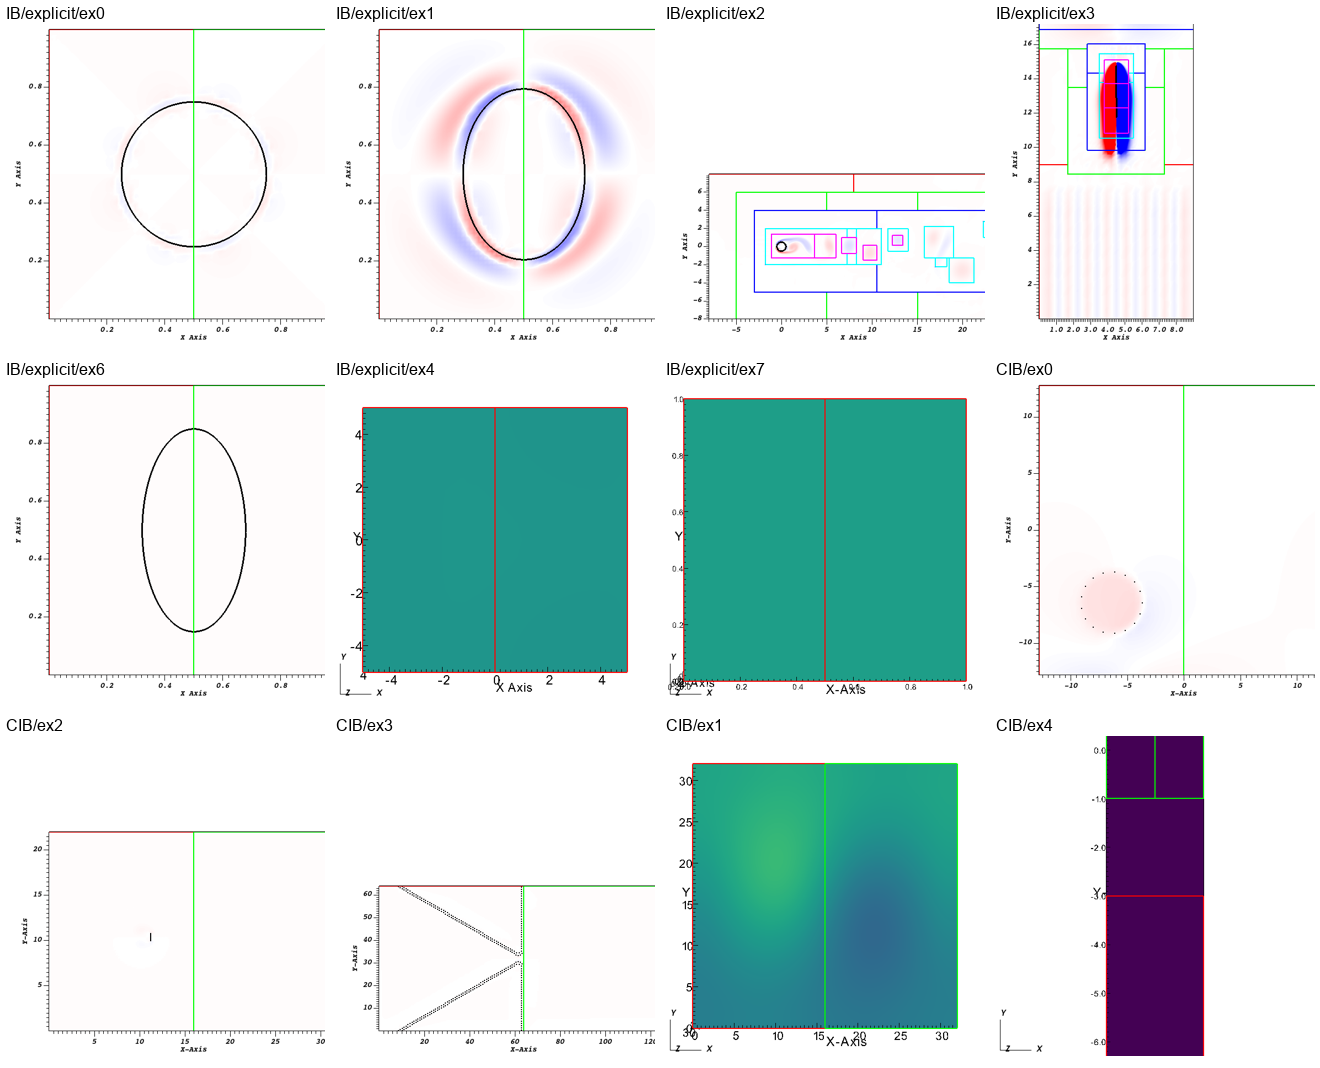
\includegraphics[width=\textwidth,height=0.74\textheight,keepaspectratio]{ch15-gallery-1}
\sourcecredit{Last saved frame of each two-minute run, rendered headless with VisIt 3.5 (chapter 26): the first of Omega, P, Q, T or the level set, with the Lagrangian mesh where there is one. Panels: IB/explicit/ex0, IB/explicit/ex1, IB/explicit/ex2, IB/explicit/ex3, IB/explicit/ex6, IB/explicit/ex4, IB/explicit/ex7, CIB/ex0, CIB/ex2, CIB/ex3, CIB/ex1, CIB/ex4.}
\end{frame}

% 26
\begin{frame}{Gallery (2)}
\label{fr:gallery2}
\centering
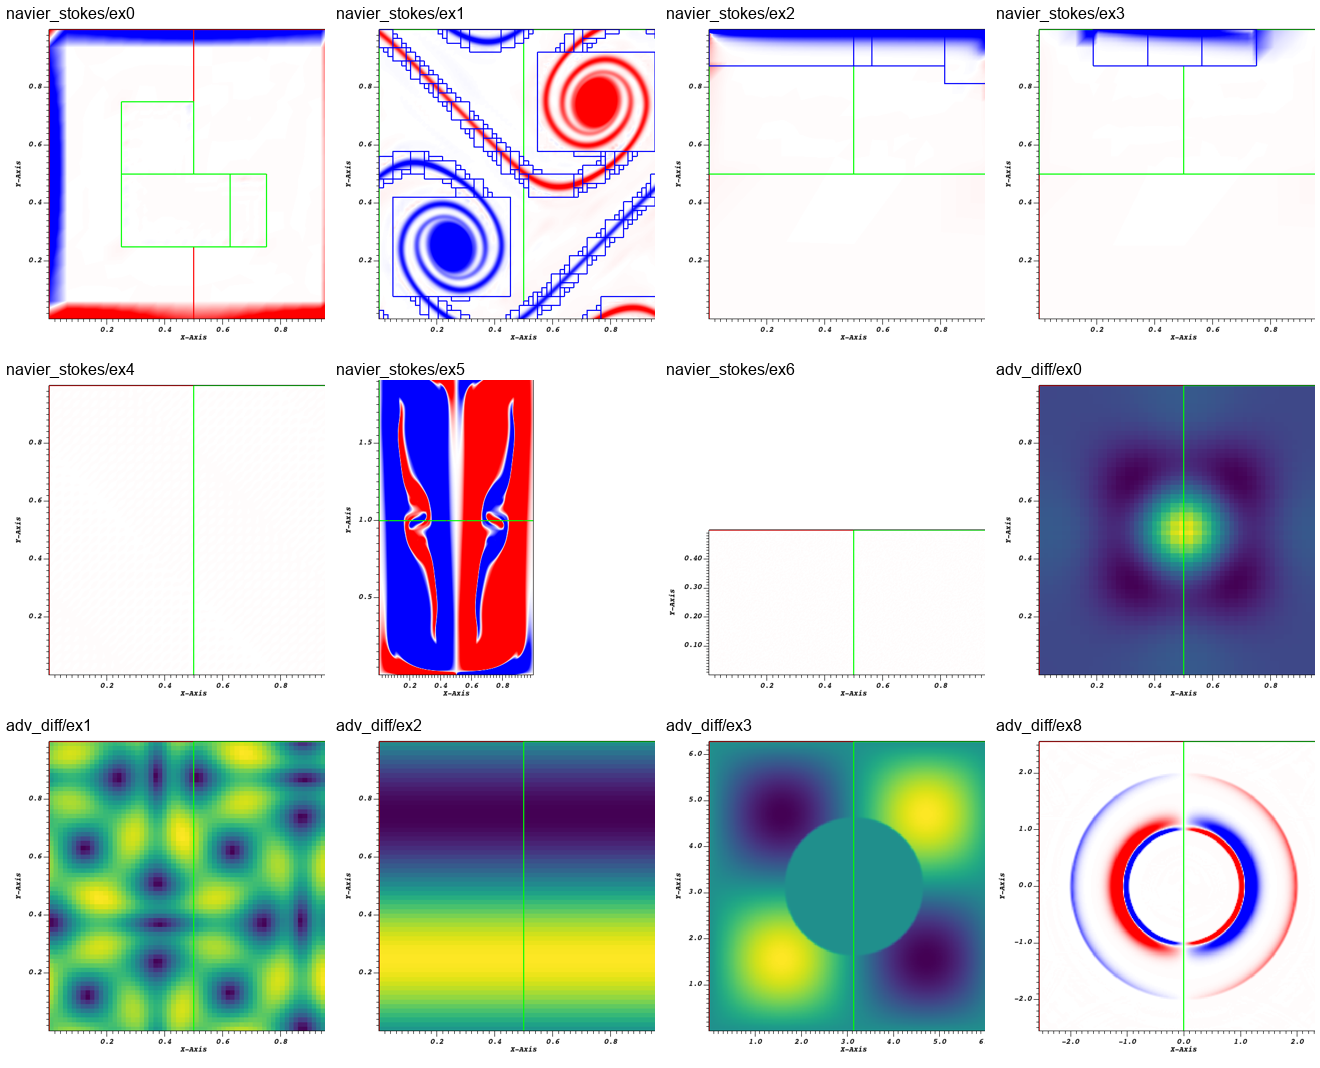
\includegraphics[width=\textwidth,height=0.74\textheight,keepaspectratio]{ch15-gallery-2}
\sourcecredit{Same rendering. Panels: navier\_stokes/ex0, navier\_stokes/ex1, navier\_stokes/ex2, navier\_stokes/ex3, navier\_stokes/ex4, navier\_stokes/ex5, navier\_stokes/ex6, adv\_diff/ex0, adv\_diff/ex1, adv\_diff/ex2, adv\_diff/ex3, adv\_diff/ex8.}
\end{frame}

% 26b
\begin{frame}{Gallery (3)}
\label{fr:gallery3}
\centering
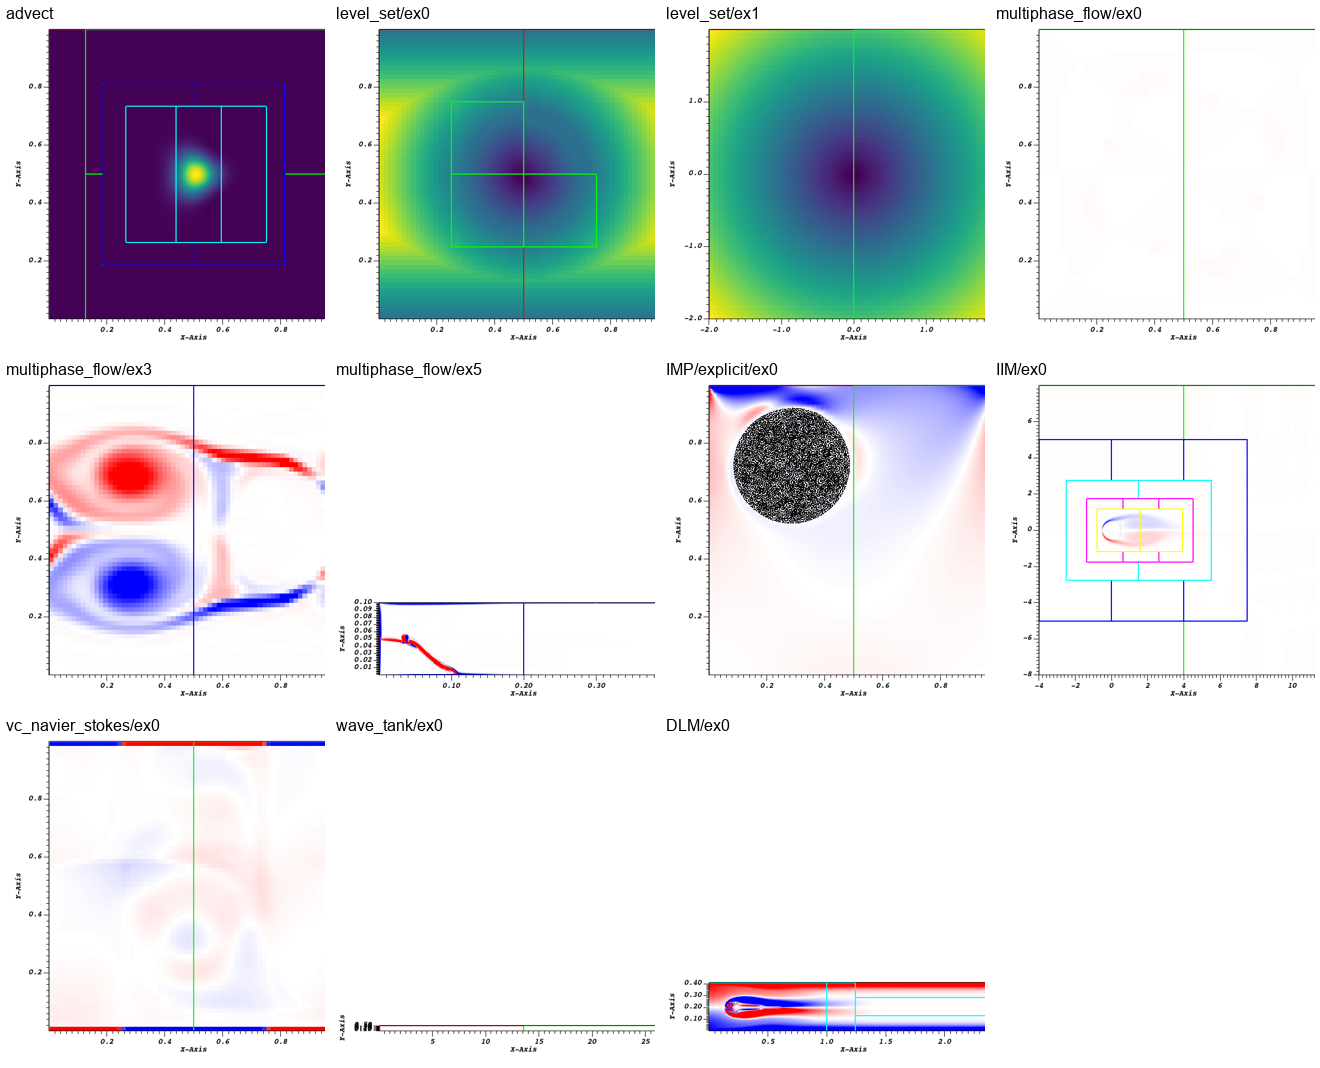
\includegraphics[width=\textwidth,height=0.74\textheight,keepaspectratio]{ch15-gallery-3}
\sourcecredit{Same rendering. Panels: advect, level\_set/ex0, level\_set/ex1, multiphase\_flow/ex0, multiphase\_flow/ex3, multiphase\_flow/ex5, IMP/explicit/ex0, IIM/ex0, vc\_navier\_stokes/ex0, wave\_tank/ex0, DLM/ex0.}
\end{frame}

% 27
\begin{frame}{Where to start, for a given problem}
\label{fr:start}
\scriptsize
\setlength{\tabcolsep}{3pt}
\begin{tabular}{@{}L{0.34\textwidth}L{0.3\textwidth}L{0.3\textwidth}@{}}
\toprule
you want to simulate & start from & then read\\
\midrule
an elastic body of fibres (a heart tube, a wing, a band) & \code{IB/explicit/ex1}, this series' IB/01 & chapters 6, 9a, 9b, 10\\
a rigid body held in a flow & \code{IB/explicit/ex2} (tethers), IB/03, IB/04 & chapters 7, 9a, 11\\
a flexible filament or flag with mass & \code{IB/explicit/ex3}, IB/12 & chapters 10, 13\\
a rigid body moving as told, or free & \code{ConstraintIB}, ConstraintIB/01--03; \code{IBLevelSet/ex1}; \code{IIM/ex4} & chapter 14\\
a swimmer with a prescribed gait & \code{ConstraintIB/eel2d}, ConstraintIB/03 & chapter 14\\
many rigid particles in Stokes flow & \code{CIB/ex1}, \code{ex4} & this chapter\\
a continuum elastic body (thick, nonlinear) & \code{IBFE/explicit/ex0}, \code{ex2}, IBFE/01 & Part IV\\
a scalar (oxygen, heat, dye) with a structure & \code{adv\_diff/ex0}, \code{ex2}; \code{IB/explicit/ex7}; IBFE/12 & chapter 24\\
a free surface, a drop, a wave & \code{multiphase\_flow/ex0}, \code{ex5}; \code{wave\_tank/ex0} & this chapter\\
a viscoelastic fluid & \code{complex\_fluids/ex0}, \code{ex1} & this chapter\\
the fluid solver's accuracy & \code{navier\_stokes/ex0}, \code{ex1}; \code{adv\_diff/ex0} with \code{converg2d} & chapter 16\\
\bottomrule
\end{tabular}
\vspace{1mm}

\scriptsize Two rules. Copy the example nearest your problem and change one thing at a time (chapter 8a). And run it first as shipped, for its shipped time or two minutes, before you change anything: the gallery slides are what ``as shipped'' looks like.
\end{frame}

% 28
\begin{frame}{What can go wrong}
\label{fr:wrong}
\scriptsize
\setlength{\tabcolsep}{3pt}
\begin{tabular}{@{}L{0.3\textwidth}L{0.36\textwidth}L{0.3\textwidth}@{}}
\toprule
what you see & why & fix\\
\midrule
\code{Cannot find source file: example.cpp} or an unknown command \code{IBAMR\_ADD\_EXAMPLE} & you configured a copied example folder with its upstream \code{CMakeLists.txt}, which only works inside IBAMR's build & the plain \code{CMakeLists.txt} of slide \ref{fr:cmake2}\\
\code{undefined reference} to a generator's \code{main}, or two \code{main}s & \code{*Gen.cpp}, \code{convergence\_tester.cpp}, \code{write\_ascii.cpp} listed with \code{example.cpp} & leave them out, or make each its own target\\
\code{Example ... requires libMesh - skipping} & IBFE, IIM, \code{multiphase\_flow/ex2}, \code{complex\_fluids/ex2}, \code{IBLevelSet/ex3} need libMesh & autoibamr builds it; check \code{IBAMR\_HAVE\_LIBMESH} in the configure log\\
the run cannot open \code{cylinder2d.vertex}, \code{petsc\_options.dat}, a \code{.e} mesh & you ran from the build folder; inputs are read relative to the working directory & run from the example folder with \code{./build/main2d}\\
the run never ends & \code{END\_TIME = 300}, $10000$, $400$ s: these are cluster jobs & shorten \code{END\_TIME}, or \code{timeout}; a Puma job for the real thing\\
the disk fills & \code{viz\_dump\_interval = 1} or restart dumps every few steps & raise the intervals (chapters 9b, 14)\\
``no flow fields'' in VisIt & the Lagrangian database was opened alone & open \code{dumps.visit} too (chapter 26)\\
\code{input2c} & the 2012 slide's typo & \code{input2d}\\
\bottomrule
\end{tabular}
\vspace{1mm}

\scriptsize Chapter 16 has the general ones (CFL aborts, parse errors, Puma limits, debugging).
\end{frame}

% 29
\begin{frame}{Homework}
\label{fr:hw}
\footnotesize
\begin{enumerate}
  \item Build and run \code{IB/explicit/ex1} with \code{input2d}, then with \code{input2d.shell} and \code{input2d.shell\_circum\_fibers}; describe in one sentence each how the three bands differ in VisIt (chapter 26).
  \item Run \code{IB/explicit/ex0}, which has no \code{.vertex} file, and find in \code{example.cpp} the function that \code{IBRedundantInitializer} calls to make the points; change the number of points and the radius.
  \item Run \code{IB/explicit/ex5} for $200$ steps and watch the free points; then set \code{kT = 0} and say what happens to them, and why the lecture's description was wrong.
  \item \code{navier\_stokes/ex2}: run the cavity for $100$ steps, then for $5{,}000$, and compare the centreline velocity with Ghia's values using the shipped \code{analyzer.m} (chapter 11 for the MATLAB side).
  \item \code{adv\_diff/ex0}: run \code{converg2d} (read it first; it runs the example at several resolutions) and report the order of accuracy you get (chapter 16).
  \item Pick the example nearest your own problem from slide \ref{fr:start}, run it as shipped for two minutes, and write down what you would change first.
\end{enumerate}
\end{frame}

% 30
\begin{frame}{Rules of thumb}
\label{fr:thumb}
\small
\begin{itemize}
  \item $98$ examples in $18$ suites; the IB ones are eight, and five of them run in seconds.
  \item Inside IBAMR's build: \code{make examples-IB}, \code{make IB-ex1}. Outside: copy the folder, drop in the plain \code{CMakeLists.txt}, link \code{IBAMR::IBAMR2d}.
  \item Run from the example folder; inputs are read from the working directory.
  \item Read \code{END\_TIME} before running: seconds for most, steps for a few, cluster-long for many.
  \item A README, when there is one, names the paper; the input's first block names the physics.
  \item ex5 is fluctuating hydrodynamics; ex0 has no vertex file; ex6 is an integrator in two files.
  \item The 2013 deck's four IB examples and four Navier--Stokes examples are still there under the same numbers.
  \item Start from the nearest example and change one thing at a time.
\end{itemize}
\end{frame}

% 31
\begin{frame}{Summary}
\label{fr:summary}
\footnotesize
\begin{enumerate}
  \item IBAMR 0.19.0 ships $98$ examples in $18$ suites: the standard IB method (8), rigid bodies three ways (CIB 5, ConstraintIB 9, DLM 1), finite elements (IBFE 12, IIM 10, IMP 1), fully Eulerian solids (IBLevelSet 7), the fluid solver alone (navier\_stokes 7, vc\_navier\_stokes 4), scalars (adv\_diff 9, advect 1), free surfaces (level\_set 2, multiphase\_flow 14, wave\_tank 2), Oldroyd-B fluids (5) and solid mechanics alone (1).
  \item They build inside IBAMR's own CMake tree as \code{examples-<suite>} and \code{<suite>-exN} targets, or outside it with a six-line \code{CMakeLists.txt} against an installed IBAMR; helper programs must be kept out of the main target.
  \item The eight IB examples: a pressurized band made in code, a bouncing ellipse and shells, a tethered cylinder with a ramped inflow, a filament with mass in a gas, a twisted 3D rod, a cloud of points in a fluctuating fluid, the band under a two-file integrator, posts with a scalar. Four of them are the course's oldest examples and this series' IB/01--IB/04 descend from them.
  \item Forty examples were built and started for this chapter; the tables and the gallery record what each did in two minutes, and which ones are cluster jobs.
  \item Three statements of the older decks are corrected: ex5's purpose, the way ex0 gets its points, and the 2012 and 2020 build recipes, which belong to trees that no longer exist.
\end{enumerate}
\begin{homebox}
\footnotesize Chapter 16 closes Part III with what can go wrong, convergence tests and debugging; Part IV opens with IBFE.
\end{homebox}
\end{frame}

% 32
\begin{frame}{What changed since the older course notes}
\label{fr:changed}
\footnotesize
\begin{itemize}
  \item The 2013/2015 deck (10 examples) and the 2020 lecture (16 examples plus ConstraintIB) are merged with the full 0.19.0 list, which is six times longer, and every suite gets at least a line.
  \item The build recipes of 2012 (\code{make examples} in a build tree that had \code{IB/staggered\_grid}), 2013 and 2020 (a Makefile with \code{make.inc} and a cluster path) are replaced by the two CMake routes, with the upstream macro quoted so that the target names are not guesswork.
  \item The examples were run, not just described: forty builds and two-minute runs, with their outcomes in the deck, and VisIt pictures from those runs instead of the 2013 screenshots (which carried desktop windows and a user name).
  \item Corrections: ex5, ex0's \code{IBRedundantInitializer}, the dead links, ``Kirchoff'', ``input2c'', and the three ``A LOT of data'' warnings, which were about \code{viz\_dump\_interval = 1}.
  \item The map from problems to starting examples (slide \ref{fr:start}) is new.
\end{itemize}
\end{frame}

% 33
\begin{frame}{Recordings (listed, not incorporated)}
\label{fr:videos}
\small The 2020 Zoom recording of IBAMR Lecture 6 (\emph{Boyce's examples}) is in the course's Drive folder and listed in the front matter's video list (chapter 0.1). The 2013 deck was taught in MATH 769 without a recording. Nothing from the recording is reproduced here.
\end{frame}

% 34
\begin{frame}{References}
\label{fr:refs}
\scriptsize
\begin{itemize}
  \item IBAMR 0.19.0, \code{examples/} and \code{examples/CMakeLists.txt}. \url{https://github.com/IBAMR/IBAMR}
  \item B. E. Griffith and S. Lim, \emph{Simulating an elastic ring with bend and twist by an adaptive generalized immersed boundary method}, Commun.\ Comput.\ Phys.\ 12 (2012) 433--461 (IB/explicit/ex4).
  \item L. Zhu and C. S. Peskin, \emph{Simulation of a flapping flexible filament in a flowing soap film by the immersed boundary method}, J.\ Comput.\ Phys.\ 179 (2002) 452--468; Y. Kim and C. S. Peskin, \emph{Penalty immersed boundary method for an elastic boundary with mass}, Phys.\ Fluids 19 (2007) 053103 (ex3).
  \item B. Kallemov, A. P. S. Bhalla, B. E. Griffith and A. Donev, \emph{An immersed boundary method for rigid bodies}, Commun.\ Appl.\ Math.\ Comput.\ Sci.\ 11 (2016) 79--141 (CIB); A. P. S. Bhalla, R. Bale, B. E. Griffith and N. A. Patankar, J.\ Comput.\ Phys.\ 250 (2013) 446--476 (ConstraintIB).
  \item R. Thirumalaisamy, N. A. Patankar and A. P. S. Bhalla, \emph{Handling Neumann and Robin boundary conditions in a fictitious domain volume penalization framework}, J.\ Comput.\ Phys.\ 448 (2022) 110726 (adv\_diff ex3--ex8); E. M. Kolahdouz et al., J.\ Comput.\ Phys.\ 2020 and 2021 (IIM).
  \item Sources: \emph{IBAMR Lecture 6: What do Boyce's examples do?} (2020, 25 slides); \emph{IBAMR Examples} (MATH 769, 2013, 18 slides; re-uploaded 2015 as tutorial 12); the 2012 lab ReadMe deck, slide 10; this series' \code{wsl/final/run\_tour.sh} and \code{visit\_tour.sh} (the forty runs and the gallery).
\end{itemize}
\end{frame}

\end{document}
